
\chapter{Discretisation induced stiffness in the Landau-Lifshitz-Gilbert equation}
\chaptermark{Discretisation induced stiffness}
\label{cha:stiffn-llg-equat}


\section{Introduction}

For continuum mechanics model of the LLG equation stiffness (the restriction of time step size by stability rather than by the desired accuracy) has long been recognised as an issue, at least for some problems \cite{Nakatani1989}.

Stiffness in PDEs has at least two possible sources:
firstly a problem may be physically stiff due to large differences in the characteristic time scales of different (physical) components of the solution \cite[Chap. 4]{Iserles2009};
secondly the choice of spatial discretisation method may cause stiffness.
In particular a fine spatial discretisation often results in a stiff system of ODEs.
An intuitive explanation for this is that a finer mesh resolves shorter wavelength modes, even if they have almost no effect on the resulting solution.
Shorter wavelength implies higher frequency, \ie shorter characteristic time scales.
These modes interact with the solution, and the large variation in time scales causes stiffness in a similar way to physical effects.
For a rigorous discussion of this effect in terms of the eigenvalues of the time integration operator see e.g. \cite[Sec 8.2]{Atkinson2009}.

As discussed in \cref{sec:time-discretisation} time integration methods can be roughly divided into two classes: those which are not good at solving stiff problems and those which are.
These two classes correspond to \emph{explicit} methods that calculate the value at the next time exclusively in terms of previous values and \emph{implicit} methods in which a system of equations must be solved.
Typically one step of an implicit method requires more computational effort than a step of an explicit method because of this solve.
However good implicit methods are unconditionally stable, allowing them to take much larger time steps when applied to stiff problems \cite[Chap. 4]{Iserles2009}.
Hence there is a trade-off between time step size and the computational effort per step.
Since the optimal choice depends on the stiffness it is important to understand its origins in micromagnetic simulations.

In \thisref{cha:stiffn-llg-equat} we examine numerically the relationship between stiffness and spatial discretisation size for a simple micromagnetic problem where stiffness due to physical effects can be ruled out.
We also explore how stiffness is affected by the use of the FEM/BEM method for magnetostatic calculations.
Finally, we study the effects of stiffness on methods which combine explicit magnetostatic calculations with implicit exchange field and LLG calculations (\ie semi-implicit methods).


\section{Problem definition}

As our example problem we chose a sphere with a radius of one exchange length.
The initial magnetisation is $\mv = [0.2, 0, 1.0]/|\mv|$, the applied field is $\happ =[0, 0, -1.1]$.
We considered three values for the Gilbert damping constant: $\alpha = 1, 0.1$ and $0.01$.
With this geometry and uniform magnetisation the magnetostatic field can be analytically shown to be $\hms = -\mv/3$ throughout the domain (as mentioned in \cref{sec:imr-ode-llg-numer-exper}) \cite[112]{Aharoni1996}, and so, due to energy considerations, the magnetisation remains uniform for spheres of radius $R < 2.082 \sqrt{3} \sim 3.606$ exchange lengths \cite[211]{HubertSchafer}.

% Note that analytically the magnetostatic field has no effect on the dynamics because it is always anti-parallel to $\mv$ (the cross product of anti-parallel vectors is zero).
The dynamics are therefore very simple: the magnetisation processes around the $z$-axis while gradually damping towards the applied field (along the negative $z$-axis).
This simplicity means that the problem can also be written as an ODE, allowing for useful comparisons.
Additionally exact solutions for the switching time are known \cite{Mallinson2000}, allowing quantification of the error.

% The spherical mesh is generated using a face splitting algorithm: begin with an icosahedron (a polygon with 20 triangular faces) then divide each face into three triangles and move the newly created node onto the surface of the sphere.
% Repeat the division to generate progressively more accurate (and expensive) approximations to the surface of a sphere.
% The list of faces is then used as input to tetgen \cite{tetgen-website} to generate an unstructured tetrahedral mesh.

As mentioned above, the simple geometry of this problem means that the physics can be captured by an ODE version of the LLG:
\begin{equation}
  \label{eq:ode-llg}
  \begin{aligned}
    \dmdt (1 + \dampc^2) &= - \mv \times \hv - \dampc \mv \times \left( \mv \times \hv \right), \\
    \hv &= \happ - \mv/3,
  \end{aligned}
\end{equation}
where $\mv = \mv(t)$.

To assess physical stiffness and find a suitable $\dtinitial$ we solved \cref{eq:ode-llg} using the RK2 and IMR methods detailed above with $\dtx{} = 0.1$.
Using IMR with $\alpha = 0.01$ we found a relative error in the final switching time of $0.3\%$ (absolute error  $1.2 \text{ time units} \approx 6\text{ps}$), for other values of $\alpha$ the percentage error is even smaller.
The relative error in switching time with $\alpha = 0.01$ using RK2 was $2.25\%$.
Since these results are from an ODE calculation the error is only due to the time integration, with no contributions from spatial discretisation.
Based on these results we conclude that $\dtinitial = 0.1$ gives a sufficiently small temporal error to be a reasonable maximum time step size.
Additionally, since no stability issues were seen for any value of $\alpha$, we conclude that any lack of stability in the PDE case must arise purely from the spatial discretisation rather than the underlying physics.

% and forward Euler needs dt=0.0001 to get comparable error!!


\section{Implementation details}

In these experiments we use the FEM discretisation of the non-dimensionalised LLG as discussed in \cref{sec:galerk-meth-llg}.
When in use magnetostatics are handled using the FEM/BEM discretisation as discussed in \cref{sec:hybr-finit-elem}.
We use three time integration schemes.
The first is the standard IMR as discussed in \cref{sec:some-implicit-time-integrators}, with monolithic coupling to the magnetostatic calculations as described in \cref{sec:fully-implicit-bem}.
The second scheme is IMR with decoupled (semi-implicit) magnetostatic calculations as discussed in \cref{sec:semi-implicit-bem}.

The third scheme is an explicit method.
For explicit time integration we use the Landau-Lifshitz form of the LLG, \cref{eq:ll-nd} because the time derivative can be written explicitly, avoiding a non-linear solve.
We use a two stage Runge-Kutta method (RK2), also known as Heun's method:
\begin{equation}
  \label{eq:heunn}
  \begin{aligned}
    \mvtemp &= \mv_n + \dtn f(t_n, \mv_n), \\
    \mv_{n+1} &= \mv_n + \frac{\dtn}{2} \left( f(t_n, \mv_n) + f(t_{n+1},
      \mvtemp) \right).
  \end{aligned}
\end{equation}
Time derivatives are calculated within the Galerkin method by inverting the finite-element mass matrix using a diagonally preconditioned conjugate gradient solver.
The magnetostatic potential $\phim$ is recalculated using the FEM/BEM method at appropriate time and magnetisation values during each stage of \cref{eq:heunn}.
The Poisson solves required for the evaluation of the potentials $\phione$ and $\phim$ use the methods discussed in \cref{sec:llg-only-system}.



Good quality (radius-to-edge ratio $ > 2$) quasi-uniform unstructured tetrahedral meshes of a sphere were generated using TetGen \cite{tetgen-website}.
Meshes were refined by decreasing the maximum element volume parameter.

All simulations were run for 4 time units ($\approx 20\text{ps}$) with a full reversal taking between 8 and 400 time units depending on the damping.
We ran the experiment without magnetostatics, with FEM/BEM magnetostatics and with the analytical magnetostatic field for each value of the Gilbert damping constant.

We use a simple heuristic algorithm to find bounds for the maximum stable step size, $\dtmax$: The computation is repeated with a sequence of decreasing step sizes (halved each time) until a stable solution is observed, with step size $\dtx{a}$. A solution is considered to be unstable if at any node $|\mv| \neq 1$ or if the maximum angle between the magnetisation of neighbouring nodes is greater than $\pi/4$. The initial step size, $\dtinitial$ is selected such that the temporal error is sufficiently small (so that any reduction in step size below this value is wasteful).

This provides bounds on the maximum stable step of $\dtmax \in [\dtx{a}, 2\dtx{a})$. To tighten these bounds we then use two steps of a standard binary search algorithm: the computation is run with $\dtn{} = 3\dtx{a}/2$, if it is successful then $\dtmax \in [\frac{3\dtx{a}}{2}, 2\dtx{a})$ otherwise $\dtmax \in [\dtx{a}, \frac{3\dtx{a}}{2})$.

\section{Results}


\begin{figure}
  \centering
  \includegraphics[width=0.8\textwidth]{images/stability_disabled}
  \caption{Maximum stable time step against discretisation size for LLG without magnetostatics. Data points are the stable dt values found, error bars represent the range in which the largest stable time step is contained. The horizontal dashed line shows the time step where RK2 and IMR are equally efficient (IMR is more efficient when the maximum stable step of the RK2 method moves below this line). The maximum time step is limited to 0.1 for accuracy reasons.}
  \label{fig:no-hms-stability}
\end{figure}


The results of the experiments with $\hms = \zerov$ are shown in \cref{fig:no-hms-stability}.
Results with full FEM/BEM magnetostatics and results with the analytical formula for magnetostatics are shown in \cref{fig:hms-stability} and \ref{fig:analytic-hms-stability} respectively.

In all cases we find that as the damping constant is reduced by an order of magnitude, stable explicit time step sizes are reduced by approximately a factor of two (due to an increase in the stiffness).

\begin{figure}
  \centering
  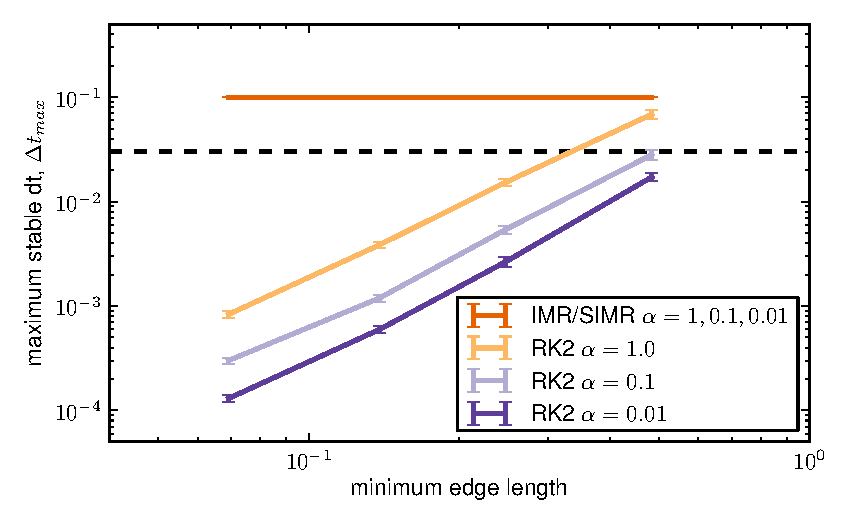
\includegraphics[width=0.8\textwidth]{images/stability_decoupled}
  \caption{Stable time step against discretisation size for LLG with FEM/BEM magnetostatics.}
  \label{fig:hms-stability}
\end{figure}


\begin{figure}
  \centering
  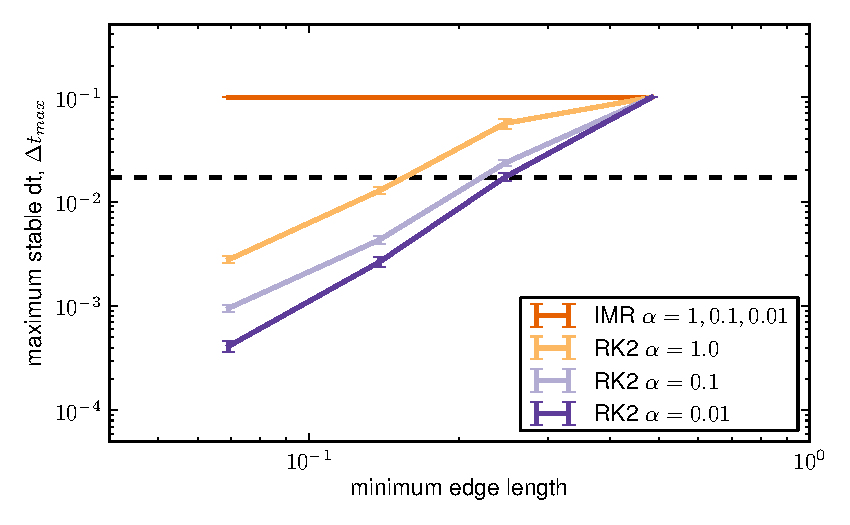
\includegraphics[width=0.8\textwidth]{images/stability_sphere}
  \caption{Stable time step against discretisation size for LLG with $\hv_{\text{ms}} = - \mv / 3$.
  }
  \label{fig:analytic-hms-stability}
\end{figure}

Comparing \cref{fig:no-hms-stability} and \ref{fig:hms-stability} we see that using FEM/BEM magnetostatics significantly increases the stiffness, requiring roughly an order of magnitude smaller explicit time steps.
However, from \cref{fig:analytic-hms-stability} we see that adding the exact field does not induce stiffness, so we can conclude that this effect is due to the FEM/BEM discretisation and not the magnetostatic field itself.
From our data we cannot predict whether other methods of calculating the magnetostatic field, such as multipole methods, will result in similar increases in the number of explicit time steps required.
However we expect that the effect is due to the coupling with the additional Poisson problems, thus any potential based method is likely to exhibit similar behaviour.

\cref{fig:hms-stability} shows that using a semi-implicit method with explicit magnetostatic calculations (SIMR) imposes no stability restrictions on the time step due to spatial discretisation for the spatial resolutions required for micromagnetic problems.

To further analyse our results we need an estimate of the ratio of computational effort for explicit vs implicit time steps. Without magnetostatics we find that each step of IMR takes on average 5.86 times more computation time than a step of RK2. With magnetostatics each step of SIMR only takes 3.40 times more computation time than a step of RK2 (the difference is due to the cost of solving multiple Poisson problems at each Runge-Kutta stage). Using these ratios we can calculate the stable RK2 time step required to have equivalent computational efficiency to IMR with step size 0.1. This stable step size is marked on \cref{fig:no-hms-stability}, \ref{fig:hms-stability} and \ref{fig:analytic-hms-stability} with a dashed line.

Based on these results we say that a problem is ``stiff'', and that an implicit method will perform significantly better than an explicit one, if the ratio of the desired time step, $\dtinitial$ to the maximum stable explicit time step, $\dtmax$ is greater than 20.
% This roughly agrees with the results of Suess \etal \cite{Suess2002}, who used the widely used (and presumably heavily optimised) CVODE package to solve the \mumag standard problem 4 using similar techniques to ours. % Their bdf2 steps are extremely slow, probably bad preconditioner.
A caveat is that both types of model could be further optimised using, for example parallelism, improved preconditioning, mass lumping, boundary matrix compression \cite[Sec. 3]{Knittel2011} etc.

Typical advice for the number of elements per exchange length is that an absolute minimum number is one, and in order to show that the results are mesh independent the mesh should be refined a few times \cite[Sec. 11]{nmag-manual}.
This leads to a reasonable finest mesh with around three elements per exchange length.

We see that with FEM/BEM magnetostatics, realistic damping ($\alpha = 0.01$) and at least three elements per exchange length the problem is stiff.

Without FEM/BEM magnetostatics stiffness only occurs if refinement to around five or more elements per exchange length is needed for any part of the domain.
Problems that require this level of refinement include resolving the geometry in studies of granular or patterned media \cite{Suess2002} and resolving vortex-core-like structures \cite{Andreas2014}.
% ??ds also \cite[App. D]{Knittel2011} found he needed this level of refinement for some parts of model to be accurate.

On the other hand LLG problems can be only moderately stiff if refinement is only needed up to the level of a few elements per exchange length, as is often required for simple geometries.
This is consistent with the fact that the mu-mag standard problem 4 is often solved using explicit integration methods with spatial refinement of around 0.5 exchange lengths \cite{mumag-website}.

Similar experiments with the standard 4th order Runge-Kutta method \cite[41]{Iserles2009} and $\alpha=1.0$ (plots not shown) give essentially the same results as for RK2. As $\alpha$ is reduced the maximum stable step size $\dtmax$ is reduced, but not as rapidly as for RK2. However due to the increased computational cost per time step (a factor of two) the onset of stiffness (for all $\alpha$) occurs at roughly the same spatial discretisation as for RK2 with $\alpha = 0.1$.

Finally we point out that the discussion above assumes that the accuracy obtained with $\dtx{} = \dtinitial$ is sufficient.
If higher accuracy than this is required then smaller time steps are needed regardless of stability, so the limitations imposed by stiffness are proportionally less significant.


\section{Conclusions}
Our results show that the LLG equation without magnetostatics or with analytical magnetostatic field calculations becomes stiff (\ie implicit methods are significantly more efficient) as the number of elements per exchange length decreases below around 5.
If FEM/BEM magnetostatic calculations are used stiffness occurs at much coarser discretisations, beginning at around $2\dash 3$ elements per exchange length.
In all cases decreasing the damping constant also increases the stiffness.

The results for the ODE version of the problem indicate that the observed stiffness is a result of the spatial discretisation and not the physics of the problem.
Since more complex physics is unlikely to reduce the stiffness, we expect that these results will extend to other, more complex, problems.

We also found that our semi-implicit FEM/BEM method does not suffer from discretisation induced stiffness.


%%% Local Variables:
%%% mode: latex
%%% TeX-master: t
%%% End:
